%\documentclass[referee]{aa} % for a referee version
%\documentclass[onecolumn]{aa} % for a paper on 1 column  
%\documentclass[longauth]{aa} % for the long lists of affiliations 
%\documentclass[letter]{aa} % for the letters 
\documentclass{aa}

\usepackage{txfonts}
\usepackage{natbib}

\usepackage{graphicx}

\usepackage{color}
\usepackage{hyperref}
\hypersetup{colorlinks=true,allcolors=[rgb]{0,0,0.8}}


\usepackage{showyourwork}

% the three lines suppress the hyperref 'link empty' warnings
% explanation at: https://tex.stackexchange.com/questions/345764/journal-class-shows-package-hyperref-warning-suppressing-link-with-empty-targe
\makeatletter
\renewcommand*\aa@pageof{, page \thepage{} of \pageref*{LastPage}}
\makeatother

\usepackage{xspace}

\newcommand{\asas}{ASASSN-21qj}
\newcommand{\ktwo}{\textit{K2}}
\newcommand{\kms}{km~s$^{-1}$\xspace}
\newcommand{\ms}{m~s$^{-1}$}
\newcommand{\gcc}{g~cm$^{-3}$}
\newcommand{\masyr}{mas~yr$^{-1}$}
\newcommand{\err}{\textit{$\pm$}}
\newcommand{\teff}{$T_\mathrm{eff}$}
\newcommand{\msun}{$M_\odot$}
\newcommand{\rsun}{$R_\odot$}
\newcommand{\lsun}{$L_\odot$}
\newcommand{\rhosun}{$\rho_\odot$}
\newcommand{\mstar}{$M_*$}
\newcommand{\rstar}{$R_*$}
\newcommand{\lstar}{$L_*$}
\newcommand{\rearth}{$R_\oplus$}
\newcommand{\vrad}{$v_{R}$}
\newcommand{\pmra}{$\mu_{\alpha}$}
\newcommand{\pmdec}{$\mu_{\delta}$}

\newcommand{\rhostar}{$\rho_*$}
\newcommand{\mjup}{$M_\mathrm{Jup}$}
\newcommand{\galex}{\textit{GALEX}}
\newcommand{\gaia}{\textit{Gaia}}
\newcommand{\kepler}{\textit{Kepler}}
\newcommand{\spitzer}{\textit{Spitzer}}
\newcommand{\ktwosc}{\textsc{k2sc}}
\newcommand{\ktwosff}{\textsc{k2sff}}
\newcommand{\hipparcos}{\textit{Hipparcos}}
\newcommand{\tess}{\textit{TESS}}
\newcommand{\emcee}{\textsc{emcee}}
\newcommand{\python}{\textsc{python}}


\begin{document} 

   \title{The eclipse of ASASSN-21qj}

   \author{M. Kenworthy
          \inst{1}
          \and
          Arttu Sainio
          \inst{2}
          \and
          Eric E. Mamajek
          \inst{3}
          \and
          Joeseph Masiero
          \inst{4}
          \and 
          Amy Mainzer
          \inst{4}
          \and
          Joeseph (Davy) Kirkpatrick
          \inst{4}
          \and 
          Richelle F. van Capelleveen
          \inst{1}
          \and
          Grant M. Kennedy
          \and
          Ludmila Carone
          \and
          NEOWISE authorship list
          \inst{4}
          \and
          AAVSO observers
          \and
          St\'{e}phane Charbonnel
          \and
        Olivier Garde
        \and
        Pascal Le D\^{u}
        \and
        Lionel Mulato
        \and
        Thomas Petit
          }

   \institute{Leiden Observatory, University of Leiden,
   PO Box 9513, 2300 RA Leiden, The Netherlands\\
   \email{kenworthy@strw.leidenuniv.nl}
         \and
             Arttu's address\\
    \and
    JPL
    \and
    Caltech/IPAC, 1200 E California Blvd, Mail Code 100-22, Pasadena, CA 91125, USA
    \and
    NEOWISE
    \and
    AAVSO people
    \and
    Space Research Institute, Austrian Academy of Sciences, Schmiedlstrasse 6, A-8042 Graz, Austria
}
   \date{Received XXXX; accepted XXXX}

% \abstract{}{}{}{}{} 
% 5 {} token are mandatory
 
  \abstract
  % context heading (optional)
  % {} leave it empty if necessary  
   {Collisions occur between planetessimals that generate debris disks through collisional cascades.}
  % aims heading (mandatory)
   {We analyze the dust and size distribution of the eclipse seen towards \asas.}
  % methods heading (mandatory)
   {Fit the light curve from three different colours to determine the particle size and distribution.}
  % results heading (mandatory)
   {The eclipse is coloured, indicating dust.
   %
   The dust has a lower limit mass of XXXX Earths, eclipse has a duration of XXXX days.}
  % conclusions heading (optional), leave it empty if necessary 
   {}

   \keywords{giant planet formation --
                $\kappa$-mechanism --
                stability of gas spheres
               }

   \maketitle
%
%-------------------------------------------------------------------

   \section{Introduction}

Terrestrial planets are thought to be built up by the quasi-periodic accretion of planetary embryos that generate a significant amount of ejected material.
%
The Earth's moon is believed to have formed from the resulting aftermath of a collision in the early Solar system.
%
Sudden increases of infrared flux from systems known to host debris disks indicate that this is a stochastic process that can occur on timescales of a few months or less.
%
Models of these impacts and the subsequent evolution of the dust clouds have been modeled \citep{Jackson12,Jackson14} and have been seen ar IR wavelengths \citep{Su19,Su22}.

The star 2MASS J08152329-3859234 underwent a sudden dimming event in December 2021, which was announced by \citet{RizzoSmith21} and assigned the identifier \asas, which we will subsequently use for the rest of this paper.
%
The star has undergone rapidly fluctuating photometry through to August 2022 \citep{RizzoSmith22} and has been monitored intensively by the AAVSO observers and the LCOGT network of telescopes.
%
It had previously shown no significant stellar variation in the optical bands for 2300 days as reported in \citet{RizzoSmith21}.
%
Searches through other photometric archives showed no other significant changes in the optical bands before this epoch.
%
The wide field infrared satellite WISE has photometric imaging from 3.8 microns (band W1) through to 22 microns (band W4), and the NEOWISE survey has photometry for bands W1 and W2 for this star.
%
This star showed a significant brightening of 0.7 magnitudes in W1 and 0.8 magnitudes in W2 between two observing epochs (65000 MJD and 65120 MJD), and the IR color of the star had changed from W1-W2=0.0 to 1.2, but no significant changes in flux in the optical bands were seen during this time.
%
Some 900 days later, the dimming was seen in the optical, and the absorption is larger at shorter optical wavelengths.
%
These observations are all consistent with an event that generated a significant amount of sub-micron dust which subsequently started to transit the stellar disk.

We hypothesise that there was a collision between one or more rocky bodies in the system which generated a significant amount of dust, which has then subsequently begun to transit the star.
%
This is consistent with a late type impact between a planet and large asteroid, similar to the one that generated the Earth/Moon system.

The structure of our paper is as follows: the analysis of the star is given in Section~\ref{sec:star}, the observations are detailed in Section~\ref{sec:obs}, and we make an estimate of the physical parameters of the hypothesised dust cloud in Section~\ref{sec:dustcloud}.
%
We then place this model in the context of planet formation in Section~\ref{sec:discussion} and summarise the paper in Section~\ref{sec:conclusion}.


%%%Statistical distributions of ejecta masses from collision in \citet{Crespi21}.

%%%%Planetary embryo collisions and wiggly disks.... \citet{Watt21}.

\section{Properties of the star}\label{sec:star}

The properties of \asas\ (Gaia EDR3 source 5539970601632026752) are listed in Table~\ref{tab:Stellarprop}.
%
Photometry from various sources was compiled and analysed using the Virtual Observatory SED Analyzer \citep[VOSA; ][]{Bayo08} and the results are listed in Table~\ref{tab:Stellarprop}, showing that \asas\ is consistent with being a G2 type dwarf star.

\begin{table}
    \centering
    \caption{Properties of \asas}
    \begin{tabular}{@{}lcc@{}}
    \hline\hline
Property                               & Value                     & Ref.  \\
        \hline
         $\alpha_{ICRS}$, J2000 {[}hh mm ss{]}  & 08:15:23.30              & 1     \\
         $\delta_{ICRS}$, J2000 {[}dd mm ss{]}  & -38:59:23.3              & 1     \\
         $\mu_{\alpha}$ {[}mas yr$^{-1}${]}     & $-9.692\pm0.012$          & 1     \\
         $\mu_{\delta}$ {[}mas yr$^{-1}${]}     & $7.349\pm0.012$          & 1     \\
         $\varpi$ {[}mas{]}                     & $1.763\pm0.011$         & 1     \\
         Distance {[}pc{]}                      & $XXXX^{+6.7}_{-5.9}$     & 2     \\ 
        \hline
         $G$ {[}mag{]}                          & $13.371\pm XXXX$        & 1     \\
         $G_{BP}-G_{RP}$ {[}mag{]}              & $0.815\pm XXXX$        & 1     \\
         $G_{BP}$ {[}mag{]}                     & $13.697\pm XXXXX$        & 1     \\
         $G_{RP}$ {[}mag{]}                     & $12.882\pm XXXXX$        & 1     \\
%         $J$ {[}mag{]}                          & $12.897\pm0.026$          & 3     \\
%         $H$ {[}mag{]}                          & $12.431\pm0.024$          & 3     \\
%         $K$ {[}mag{]}                          & $12.321\pm0.024$          & 3     \\
%         $u$ (AB) {[}mag{]}                     & $17.63\pm0.02$            & 4     \\
%         $g$ (AB) {[}mag{]}                     & $16.096\pm0.008$          & 4     \\
%         $r$ (AB) {[}mag{]}                     & $16.69\pm0.02$            & 4     \\
%         $i$ (AB) {[}mag{]}                     & $14.123\pm0.005$          & 4     \\
%         $z$ (AB) {[}mag{]}                     & $14.832\pm0.011$          & 4     \\
        \hline
         $R_*$ [\rsun{}]                        & $1.009\pm0.030$           & 5     \\
%         $M_*$ [$M_{\odot}$]                    & $0.85\pm0.02$             & 5     \\
         {[}Fe/H{]} [dex]                       & $0.0\pm0.23$               & 5     \\
         log\,$g$ [log$_{10}$ cm\,s$^{-2}$]     & $4.5\pm0.25$               & 5     \\
         \teff{} [K]                            & $5900\pm74$               & 5     \\
%         $f_{bol}$ [10$^{-11}$ erg s$^{-1}$]    & $5.288\pm0.130$           & 5     \\
%         $m_{bol}$ [mag]                        & $14.194\pm0.027$          & 5     \\
         $m_{bol}$ [mag]                        & $13.39\pm0.02$           & 5     \\
%         $L_{bol}$ [$L_{\odot}$]                & $0.046\pm0.013$         & 5     \\
         log($L/L_{bol}$) [dex]                 & $0.046\pm0.013$        & 5     \\
         
        \hline
    \end{tabular}
    \tablefoot{References:
    (1) Gaia EDR3 \citep{Brown21},
    (2) \citet{BailerJones21},
    (3) 2MASS \citep{Cutri03},
    (4) SDSS DR8,
    (5) this work (EEM fits)
    }
    \label{tab:Stellarprop}
\end{table}

% Including IR WISE photometry
%was forcing it to lower metallicity ([Fe/H] ~ -0.5-1), cooler (~Sun) fits. Fits also favor low reddening values ($A_v\sim 0.05$). 
%Similar to Alpha Cen A, but ~solar metallicity seems OK now. Almost exactly 1 Rsun! 

%Best parameters as of 1/2/2022 (see below from VOSA fit) 
%Teff = 5900 +- 74 K
%log(L/Lsun) = 0.046+-0.013 
%Av = 0.05+-0.03
%mbol = 13.39+-0.02 (apparent)
%logg = 4.5+-0.25
%[M/H] = 0.0+-0.23 
%Rad = 1.009 +- 0.030 Rsun

% This SED is not from VOSA, would need one from there to match Eric's fit
% \begin{figure}
%    \centering
%    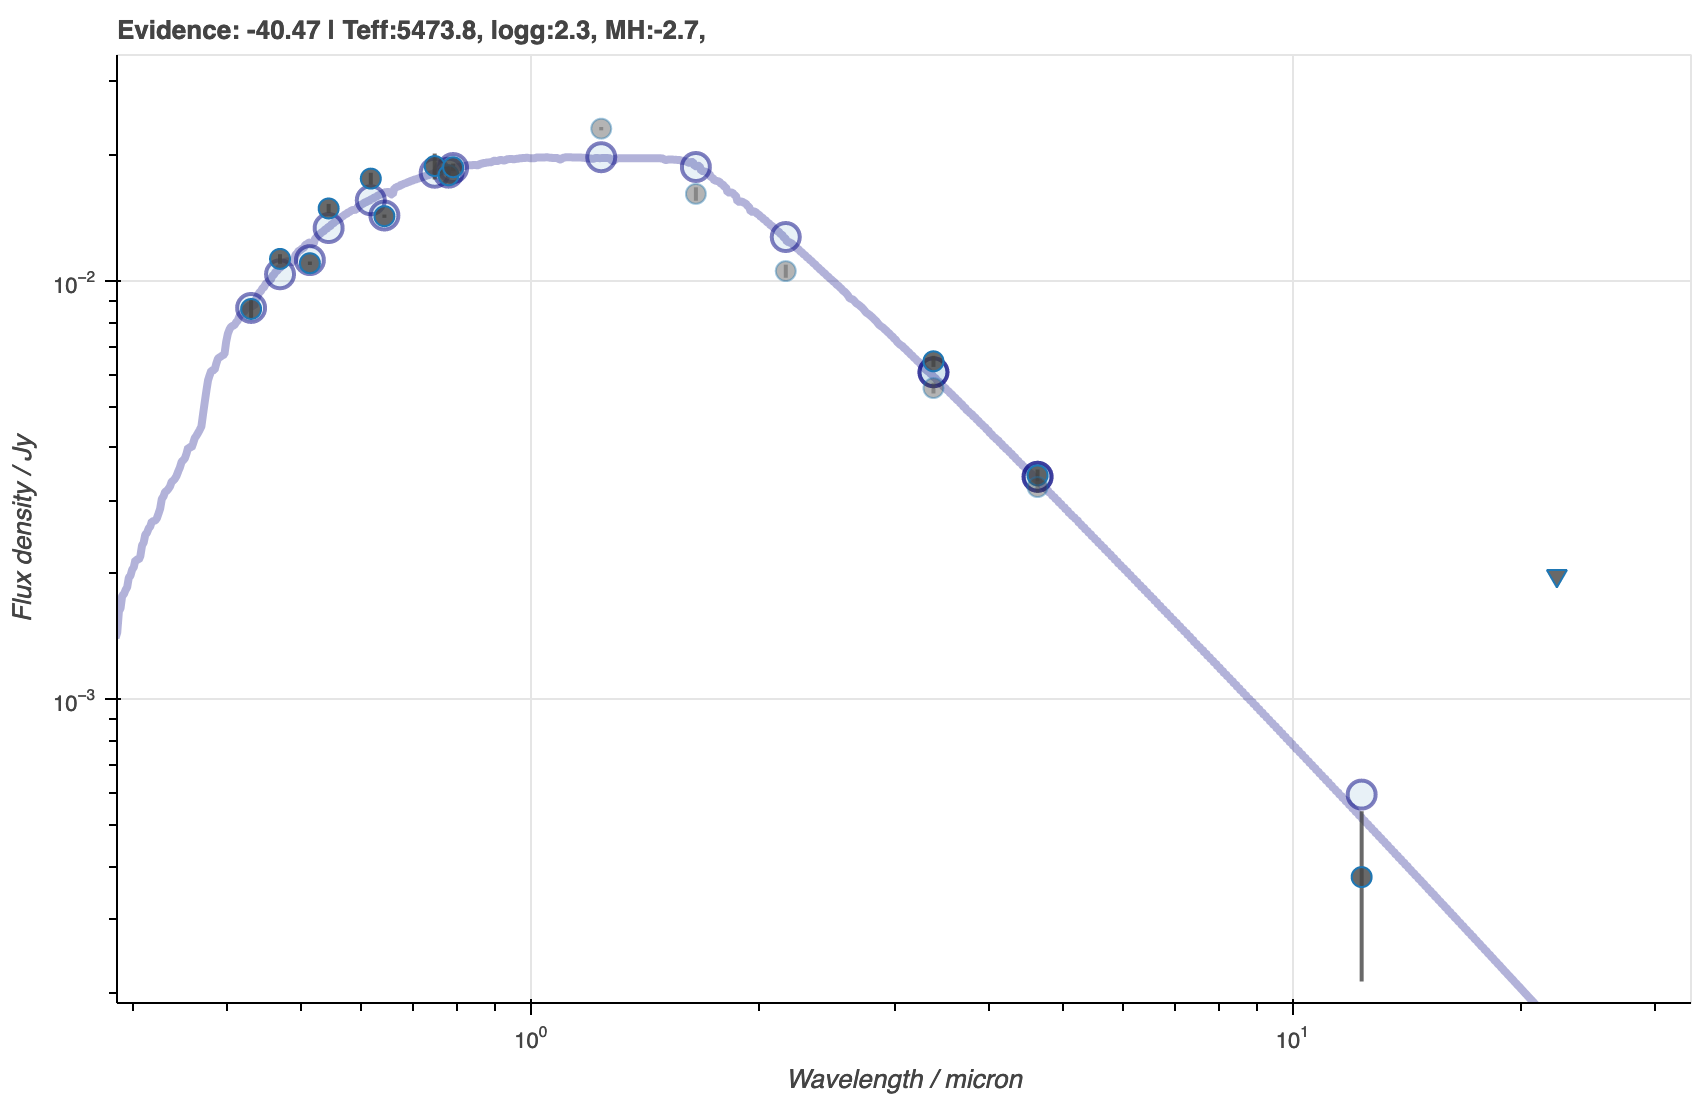
\includegraphics[width=\hsize]{figures/asassn-21qj-gmk-sed-fit.png}
%       \caption{VOSA fit to photometry of \asas .}
%          \label{fig:sed}
% \end{figure}


\begin{figure}
   \begin{centering}
   \includegraphics[width=\hsize]{figures/filter_curves.pdf}
      \caption{Filter curves for all telescopes and filters used to observe \asas.}
      \label{fig:allfilters}
      \script{plot_filter_curves.py}
      \end{centering}
\end{figure}

%\begin{figure}
%   \begin{centering}
%   \includegraphics[width=\hsize]{figures/mie_single.pdf}
%      \caption{Mie test.}
%      \label{fig:mietest}
%      \script{plot_mie_single.py}
%      \end{centering}
%\end{figure}

\begin{figure*}
   \begin{centering}
   \includegraphics[width=\textwidth]{figures/eclipse_overview2.pdf}
      \caption{Photometry from the optical bands of the eclipse.
      %
The different telescopes and filters are indicated in the legend.
%
Each light curve is offset vertically by 0.8.
              }
        \label{fig:eclipse_overview}
        \script{plot_eclipse_overview2.py}
    \end{centering}
\end{figure*}

\subsection{Possible multiplicity of \asas}

\asas\ (Gaia DR3 5539970601632026752 = 2MASS~J08152329-3859234) has a neighbor (Gaia DR3 5539970597334497024 = 2MASS~J08152298-3859244) which might plausibly be a physical companion.
%
Based on the Gaia EDR3 mean ICRS position for epoch 2016.0, the visual companion lies at a separation $\rho$ = $3738.243\pm0.062$ mas and at position angle $\theta$ = $249^{\circ}.977$.
%
Their parallaxes ($\varpi$ = $1.7631\pm0.0112$ mas vs. $1.4711\pm0.0523$ mas) differ by 5.5$\sigma$ and proper motions ($\mu_{\alpha} = -9.692\pm0.012$, $\mu_{\delta} = 7.349\pm0.012$ \masyr\, vs. $\mu_{\alpha} = -0.114\pm0.055$, $\mu_{\delta} = 6.419\pm0.053$ \masyr) differ by a factor of 2.
%
If the two stars are at the parallactic distance of \asas\ \citep[$d$ = 552.4 pc;][]{BailerJones21}, then their difference in proper motion ($\Delta\mu$ = $9.623\pm0.056$ \masyr) translates to a difference in tangential velocity of $\Delta V_{tan}$ = $25.37\pm0.21$ \kms.
%
The velocity difference is considerable given the projected separation of 2079\,au.
%
Using Kepler's 3rd law, and assuming the observed separation corresponds to the semi-major axis, and the observed $\Delta V_{tan}$ corresponded to the full orbital velocity, these quantities would predict a minimum system mass of $>150$ \msun.
%
Based on the implausible estimated dynamical mass inferred from the observed separation and difference in tangential velocities, we conclude that the visual companion 2MASS J08152298-3859244 is an interloper unrelated to \asas.

\section{Observations}\label{sec:obs}

The beginning of the eclipse was announced in \citet{RizzoSmith21} through the ASASSN survey, which triggered several observing campaigns at optical wavelengths, and an ALMA observation at Band 7 (program \texttt{2019.A.00040.S}).
%
An overview of all the photometry is presented in Figure~\ref{fig:allphot}, along with the filter passbands for all the observations in Figure~\ref{fig:allfilters}.
%
A spectrum of the star was obtained with the 2SPOT consortium midway through the eclipse.
%

\subsection{ASAS}

The All Sky Automated Survey \citep[ASAS; ][]{pojmanski_all_1997, asas_2005, asas_2018} is a survey consisting of two observing stations - one in Las Campanas, Chile and the other on Maui, Hawaii. 
%
Each observatory is equipped with two CCD cameras using V and I filters and commercial f $ = 200$ mm, D $= 100$ mm lenses, although both larger (D $= 250$ mm) and smaller (50-72 mm) lenses were used at earlier times.
%
The majority of the data are taken with a pixel scale of $\approx$ 15\arcsec{}.
%
ASAS splits the sky into 709 partially overlapping (9\degr{} $\times$ 9\degr{} fields, taking on average 150 3-minute exposures per night, leading to a variable cadence of 0.3-2 frames per night.
%
Depending on the equipment used and the mode of operation, the ASAS limiting magnitude varied between 13.5 and 15.5 mag in V, and the saturation limit was 5.5 to 7.5 mag. 
%
Precision is around 0.01-0.02 mag for bright stars and below 0.3 mag for the fainter ones. 
%
ASAS photometry is calibrated against the Tycho catalog, and its accuracy is limited to 0.05 mag for bright, non-blended stars.

\subsection{ASAS-SN}

The All Sky Automated Survey for Supernovae \citep[ASAS-SN; ][]{shappee_man_2014,kochanek_all-sky_2017} consists of six stations around the globe, with each station hosting four telescopes with a shared mount.
%
The telescopes consist of a 14-cm aperture telephoto lens with a field of view of approximately 4.5\degr{}$\times$4.5\degr{} and an 8.0\arcsec{} pixel scale.
% 
Two of the original stations (one in Hawaii and one in Chile) are fitted with $V$ band filters, whereas the other stations (Chile, Texas, South Africa and China) are fitted with $g$ band filters.
%
ASAS-SN observes the whole sky every night with a limiting magnitude of about 17 mag in the $V$ and $g$ bands.
%

\subsection{TESS}

The Transiting Exoplanet Survey Satellite \citep[TESS; ][]{2015JATIS...1a4003R} is a satellite designed to survey for transiting exoplanets among the brightest and nearest stars over most of the sky.
%
The TESS satellite orbits the Earth every 13.7 days on a highly elliptical orbit, scanning a sector of the sky spanning 24\degr $\times$ 96\degr\ for a total of two orbits, before moving on to the next sector. 
%
It captures images at a 2 second (used for guiding), 20 seconds (for 1000 bright asteroseismology targets), 120 seconds (for 200 000 stars that are likely planet hosts) and 30 minutes (full frame image) cadences.
%
The instrument consists of 4 CCDs each with a field of view of 24\degr$\times$24\degr, with a wide band-pass filter from 600-1000 nm (similar to the $I_C$ band) and has a limiting magnitude of about 14-15 mag ($I_C$).
%
The data was extracted from the TESS archive using the {\tt eleanor} package \citep{Feinstein19} which corrected for known systematics in the cameras and telescope.

\subsection{ROAD Photometry}

The Remote Observatory Atacama Desert \citep[ROAD; ][]{Hambsch12} is a fully automated telescope located in Chile that obtains nightly photometry in multiple bands for a wide range of astronomical projects.
%
It consists of a 40-cm $f/6.8$ Optimized Dall-Kirkham and uses a Finger Lakes Instruments camera with a 4k$\times$4k array with pixels of $5\mu m$ in size.
%
Data are reduced using a custom pipeline and then published on the AAVSO website.

\subsection{NEOWISE photometry}

The NEOWISE photometry is presented with the ASASSN $q$ light curve in Figure~\ref{fig:wisephot}.

\begin{figure*}
\begin{centering}
\includegraphics[width=\textwidth]{figures/all_photometry.png}
\caption{NEOWISE $W1$ and $W2$ photometry of the star, with the WISE color in the lowest panel.
%
The $NEOWISE$ color changes from colourless to very red, which fades back towards colourless over $\sim 500$ days.
}
\label{fig:wisephot}
\script{plot_all_photometry.py}
\end{centering}
\end{figure*}


\begin{figure*}
\begin{centering}
\includegraphics[width=\textwidth]{figures/stellar_lomb_scargle.pdf}
\caption{ASASSN photometry of \asas\ and the Lomb Scargle periodograms of the photometry in and out of the eclipse.
%
The blue and orange shaded regions in the top panel indicate the range of epochs put into the Lomb Scargle periodogram.
%
Middle panel: The periodograms over a range of 0 to 150 days.
%
Lower panel: The periodogram of the star outside of the eclipse over a range of 0 to 50 days.
}
\label{fig:starlombscargle}
\script{calc_stellar_lomb_scargle.py}
\end{centering}
\end{figure*}



NEOWISE....

\variable{output/collision_epoch_text.txt}


\subsection{LCOGT photometry}

\subsection{ATLAS}

ATLAS is a project that searches for near earth asteroids down to a magnitude of 19 
\citep{Tonry18}.
%
Two filters were obtained, the `o' and `c' filters respectively.
%
Photometry consists of two to four photometric points observed each night when conditions permitted.
%
Photometry with large errors was rejected in a first pass.
%
The remaining observations during a night were averaged and an error based on the r.m.s. of these nightly points was calaulated.
%
The photometry covers the time period where the collision event occurred. 

\subsection{2SPOT spectroscopy}

A spectrum of the star was taken on 59829.8785 MJD equal to 2022-09-07 at 08:34:52 UTC from the Deep Sky Chile\footnote{\url{https://www.deepskychile.com/en/}} site in Chile (at longitude:70\degr 51\arcmin 11\farcs 86
latitude:30\degr S 31\arcmin 34\farcs 71 altitude:1700m AMSL).
%
The telescope is a Ritchey-Chretien telescope ($d=305$mm) at $f/5$ (with focal reducer CCD 67 astrophysics) on an equatorial mount GM 3000 HPS from 10 micron\footnote{\url{https://www.10micron.com/en/product/gm3000-hps/}}.
%
The spectrograph is a Spectrograph Alpy 600 $R=570$ with a $23\mu m$ wide slit\footnote{\url{https://www.shelyak.com/produit/alpy-600/?lang=en}} and an ATIK 414ex camera\footnote{\url{https://www.atik-cameras.com/product/atik-414ex/}}.
%
The spectrum is composed of three unbinned exposures of 1200s each, taken in automatic mode with Prism V11 Software (https://www.prism-astro.com/) , spectrum process with ISIS software\footnote{\url{http://www.astrosurf.com/buil/isis-software.html}}.
%
The final spectrum is shown in Figure~\ref{fig:2spotspectrum}.

%And for more informations about 2SPOT, you wil find many informations in our website : https://2spot.org/EN/
%and also information about the team : https://2spot.org/EN/equipe.php


\begin{figure*}
   \begin{centering}
   \includegraphics[width=\textwidth]{figures/2spot_spectrum.pdf}
      \caption{Spectrum of \asas\ showing features of a typical G type star.
              }
              \label{fig:2spotspectrum}
              \script{plot_2spot_spectrum.py}
              \end{centering}
       \end{figure*}

\subsection{ALMA}

The ALMA data were downloaded and processed through to a measurement set with CASA \citep{2007ASPC..376..127M}.
%
No source is visible in the default archive products, and we also detect no source at the expected location in CLEAN images.
%
We measure a source flux of $X \pm y$\,mJy, equivalent to an upper limit of $Z$\,mJy.
%
In terms of the infrared excess visible in the mid-IR with WISE this upper limit is not at all constraining, but does set limits on emission from cooler dust.
%
These limits are not particularly constraining either, with $L_{\rm dust}/L_\star \gtrsim 10^-3$ at $\sim$100\,K detectable (which for context is approximately the level seen for the very bright debris disk around $\beta$~Pictoris).

\section{Analysis}\label{sec:dustcloud}

\subsection{Dust properties from the colors in the optical}

{\bf Richelle plots}: The photometry shows deeper absorption at bluer wavelengths compared to longer wavelength passbands.
%
This is an indication that the stellar flux is being scattered by particles that are equal to or smaller than the wavelength of light.
%
By plotting the magnitude of the star versus colour (e.g V versus V-I) the particle size and surface density can be determined.
%
Plots of the light curve show reddening concistent with interstellar dust, and this reddening is parameterised with a reddening angle (Richelle: I'm not sure of the correct name for this!)

The sampling of the photometry enables determination of the reddening as a function of time during the eclipse.
%
The reddening is calculated in 20 day bins and plotted in Figure ZZZZ, showing that the reddening angle is very consistent over the duration of the eclipse, but that there is a suggestion that the reddening angle changes gradually during the ingress and egress.

TODO: to estimate the minimum mass of all the sub-micron dust in the eclipse and equate that to YYYYY kg of solid material.

\subsection{Transverse velocity of the dust cloud}

The photometry changes with time, and this is attributed to a cloud of dust moving in front of the stellar disk at a velocity $V_{dust}$ and that has a surface density that changes as a function of position in the dust cloud.
%
A lower bound can be derived for $V_{dust}$ by measuring the gradient of the light curve and determine what velocity a sharp edged and completely opaque occulter moving across the disk of the star would be need to make the same gradient.

We measure the gradient of the light curve in an automated way by fitting straight lines to photometry between nights (XXX Richelle correct me on this!)
%
We determine a robust lower limit to the transverse velocity of 5 km\,s$^{-1}$ for the material moving in front of the star, assuming a radius for the star of $1.07 R_\odot$.
%
This means that if the dust is on a circular orbit, it has to be within XXX au equivalent to an orbital period of YYY years around the star.

\subsection{Frequency analysis of the light curve}

To search for signs of periodicity within the light curve before and during the eclipse, we perform a Lomb-Scargle analysis over two epochs indicated with the blue and orange regions in the upper panel of Figure\~\ref{fig:starlombscargle}.
%
The resultant periodograms are shown in the lower two panels of Figure\~\ref{fig:starlombscargle}, with the lower panel showing a zoom in from 0 to 50 days and the middle panel showing periodicities from 0 to 150 days.
%
We look for any perioditicies that could be associated with orbital motion aorund the star, so we look at the periodogram from 0 to 150 days during the eclipse.
%
As a comparison, we overplot the periodogram for the pre-eclipse light curve as the blue curve in the middle panel. 
%
As can be seen, there is some power seen at 40 days which is present in the pre-eclipse light curve, with some (non-significant) periodicities at longer periods.

Looking for periodic stellar activity, the periodogram for the pre-eclipse light curve is shown from 0 to 50 days in the lower panel.
%
Here we see significant periods at around 6.5 and 11 days, which we attribute to light curve modulation due to starspots rotating in and out of view. 


\begin{figure*}
   \begin{centering}
   \includegraphics[width=\textwidth]{figures/scale_combined_photometry.pdf}
      \caption{Photometry from the optical bands of the eclipse scaled arbitrarily so as to combine the light curves into a ``gray'' light curve.
      %
      The axis is inverted to show Absorption.
              }
              \label{fig:allphot}
              \script{plot_scale_combined_photometry.py}
              \end{centering}
       \end{figure*}



\section{Discussion}\label{sec:discussion}

We have two separate phenomena that occur within 1000 days of each other.
%
Firstly, NEOWISE W1 and W2 photometry towards the star shows an increase in flux of a factor of two in both wavebands, with the longer wavelength showing a larger increase.
%
Observations from the optical bands have a much higher cadence, but do not show any corresponding increase in flux.
%
This infrared only increase is consistent with a dust generating event, such as the collision of a planetoid with another planetoid or a terrestrial planet (REF REF).
%
This interpretation is also supported by the reddening of the star during the optical dimming, if we assume that both the optical and IR flux variations are caused by the same dust (discussed further below).
%
The resultant dust cloud has a considerably larger surface area than the progenitors (which were not visible before the IR flux increase), and this dust cloud is then heated by some luminosity source.
%
Typically the host star heats circumstellar dust, but we consider alternative possibilities below.
%
% The temperature of the dust cloud can be estimated from spectral energy distribution (SED) measured towards the stellar system. A post-increase SED is shown in Figure \ref{fig:sed-after}, using WISE data from the first five post-increase epochs, for which the best-fit dust temperature is $910 \pm 50$\,K. This temperature is consistent with those derived from the time series, though more precise because the data have been averaged.

% \begin{figure}
%     \centering
%     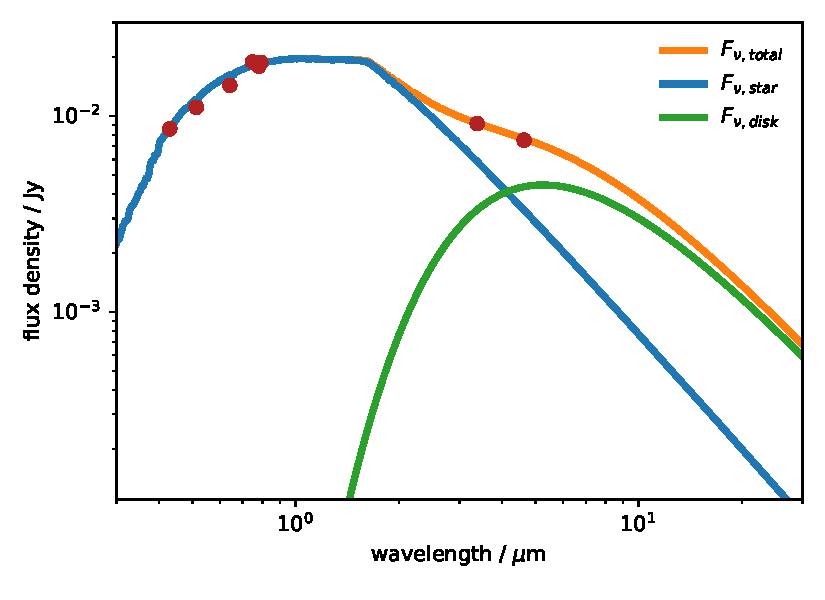
\includegraphics[width=1\textwidth]{figures/asassn-21qj-after.pdf}
%     \caption{SED of \asas~after the IR flux increase. The blue line shows the stellar photosphere model, the red line the dust model (a blackbody), and the orange the total.}
%     \label{fig:sed-after}
% \end{figure}

\subsection{Scenario independent constraints}

We first consider some scenario independent constraints, as these illustrate some basic problems which are summarised in Figure \ref{fig:constr}.
%
Most simply, the IR photometry requires very warm dust, but the delay between the IR flux increase and the optical dimming suggests material that is far from the star.
%
While there are other means that stellar luminosity to heat dust, the star is the most conventional source, and requires the dust to be at about 0.1\,au.
%
A several-year delay between the IR flux increase and the optical transit however implies that the material is on an orbit with a period of at least several years, and hence several au.
%
The duration of the optical transit also suggests a distance of order an au or greater, since closer material would have a period that is shorter than the duration of the transit.
%
Finally, a large orbital distance is also suggested by the gradients in the optical light curve, though the velocities inferred from the gradients are lower limits and hence the material could be closer.

Thus, if the IR and optical flux varaitions have the same origin, there are basic incompatibilities for scenarios that assume an azimuthally confined clump of orbiting material that is heated by the star.
%
Possible explanations therefore attempt to avoid these restrictions.

\begin{figure}
    \centering
    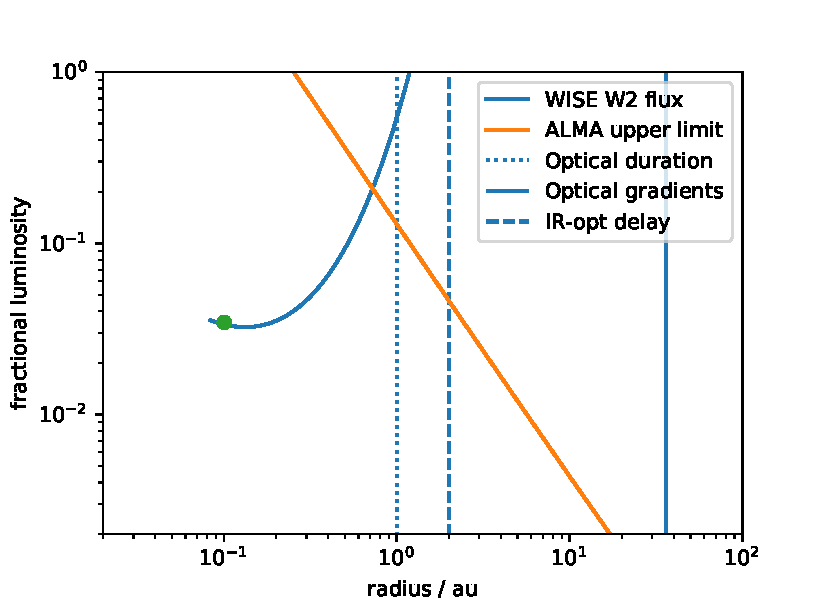
\includegraphics[width=0.5\textwidth]{figures/fvsr.pdf}
    \caption{Model-independent constraints in terms of dust fractional luminosity ($L_{\rm dust}/L_\star$) and stellocentric radius.
    %
    The dot shows the location of the dust from an SED fit, and the curved line shows cooler dust that is consistent with the WISE W2 flux alone.
    %
    The diagonal line shows the upper limit from the ALMA non-detection.
    %
    The vertical dotted line shows an approximate lower radial limit on the dust location based on the transit duration.
    %
    The dashed line a lower radial limit based on the delay between the IR flux increase and optical transit.
    %
    The vertical solid line shows an upper radial limit based on the optical light curve gradients.}
    \label{fig:constr}
\end{figure}

This increase occurred between MJD \variable{output/t_before.txt} and MJD \variable{output/t_after.txt} dates, a period of approximately \variable{output/t_duration.txt} days.
%
Subsequent NEOWISE measurements show an approximately constant excess flux for XXXX days, followed by a decrease from XXXX to XXX.

We fit a blackbody SED to the excess flux in the two NEOWISE bands for each of the epochs.
%
Assuming grey emission (where $\upsilon(\lambda)\approx \upsilon$) we obtain an effective temperature of $_{IR} = 900\pm XXX$K, and $F_{IR}/F_{star}=0.03$. Given the near-Solar luminosity of the star, this temperature implies a distance of approximately 0.1\,au if the material absorbs and emits as a blackbody, and of order a few times more distant if it is micron-sized dust (e.g. Pawellek). 
%
The sudden onset of the IR flux within 155.21 days followed by a constant level of flux implies that the dust cloud reaches a (quasi) steady state within 6 months, though could be optically thick or thin.
%
Regardless, the dust distribution has had to expand such that 0.03 of the solid angle around the star was subtended by dust and reradiated in the IR.
%
An estimate for the surface area $A_{IR}$ of the dust can be estimated from $A_{IR}/(4\pi r_{IR}^2) = 0.03$ which leads to:

$$A_{IR}=0.38 r_{IR}^2$$ 

where $r_{IR}$ is the distance of the dust from the star.

Hansen collision of terrestrial planet with scattered moon \citep{2022MNRAS.tmp.2636H}

Cound be a ring system

Alternatives?

\textcolor{magenta}{Probing disintegrating planetary material has been proven to be a very useful method to access the composition of building blocks of planets outside of the Solar System.
%
E.g. the disintegration of a gas giant around a white dwarf was used to infer its composition \citep{Gaensike2019}.
%
White dwarf star pollution has also yielded insights about refractory (Fe/Mg/Ca) element content of rocky  material around such stars \citep{Turner2020,Putirka2021,Blouin2020}.
%
See also \cite{Veras2021} for a review.}

\textcolor{magenta}{Planets and asteroids falling into white dwarfs, however, haven been probably heavily processed during the late stellar evolution.
%
The unusually warm (how much?) debris disk passing in front of a young star presented in this work, on the other hand, may allow to probe the interior of planetesimals in the early stages of planet formation.
%
The eclipse is expected to last for xxx days, allowing to perform further spectroscopic analysis of the dust in this system.}

\subsection{HYP 1: unrelated phenomena} 

As discussed below, the observations pose some problems regarding the location of the occulting cloud. The long timescale between the WISE flux increase and the optical dimming, and the gradients in the optical light curve, suggest that the dust is of order au away from the star. This however is contradicted by the hot dust temperature, which would place the dust near 0.1\,au. Important here is that the system first came to prominence because of the optical variability, even though subsequent investigation found that the IR flux increase occurred beforehand.

A possible resolution is simply that the WISE flux increase and the optical dimming are unrelated coincidental phenomena. This explanation is unsatisfactory however, because both IR flux increases and dimming events are rare, particularly around stars that are not young. For example, constant near-IR excesses are exceptionally rare among main-sequence stars (1:10,000), and still uncommon for young stars \citep[1:100][]{2013MNRAS.433.2334K}. In addition, these rates are for 12$\,mu$m excesses that are largely constant; rates are lower at shorter wavelengths, and no star has been seen to show an increase from no excess to a sizeable excess \citep[][report a disappearing mid-IR excess, but this is the single example known]{2012Natur.487...74M}. Work has shown that young stars that do have unusually bright mid-IR excesses do have a high probability of showing IR flux variability \citep{2015ApJ...805...77M}, which suggests that \asas~could be a young system.

Similarly, optical dimming events are also rare for main-sequence stars, for example only one was seen to undergo dust-related optical dimming with Kepler \citep{2016MNRAS.457.3988B}. Young stars that host protoplanetary disks do regularly show optical dimming (known as ``dippers''), but these generally have large and constant mid-IR excesses \citep[e.g.][]{2016ApJ...816...69A}.

While it is hard to estimate the total probability of observing such a system, we can estimate that the probability of a random star that shows unusual optical dimming also having a mid-IR excess is at best 1\% if the system is young, and much lower if it is not. Not all mid-IR excess systems are variable, but quantifying the probability of variability is not simple, so we simply conclude that the coincidental optical and mid-IR flux variation is a best an order 1\% event, but probably much less probable.

\subsection{HYP 2: dust heated by star}

If one insists that the dust is heated by the star, then as noted above it must be relatively close to it; too close for the delay between the IR flux increase and the optical flux decrease to be explained as a fraction of the orbital period. For example, for material at 0.1\,au the orbital period is a few weeks. While we may still invoke some singular event to explain the increase in IR flux, e.g. a collision, the new material will rapidly shear azimuthally into a disk, and the optical dimming must then be explained by variation over multiple orbital timescales.

The lack of significant variation in the WISE flux after the increase suggests that this shearing has largely happened within a period of six months. A longer timescale should lead to behaviour that is similar to that seen for stars such as ID8 \citep{2014Sci...345.1032M}, while the material is still shearing and has significant azimuthal variation. Thus, any changes that lead to occultation of the star are more likely related to changes in vertical structure of the disk. Such an increase could be caused by continued dynamical interactions between the massive debris, or excitation by a single larger body \citep[e.g.][]{1992Icar...96..107I}.

A possible scenario is therefore that the debris was created in a collisional event involving one or two large bodies, resulting in a sizeable debris cloud. With respect to the collision center of mass, this cloud leaves with at least the escape velocity from the larger body, and is sheared out over tens of orbital periods. The random velocities of the debris cloud objects are then further increased by dynamical interactions (``stirring'') both between fragments, and by the original large bodies, the main relevant effect being that the scale height of the disk will slowly increase.

To satisfy the observational constraints, the system must be near to edge-on, such that the disk does not initially block the star. Over time however, the increase in scale height begins to block the star, leading to the slow decrease in optical flux. The depth of the optical dimming implies that the disk was initially radially optically thick. The radial optical depth must now be decreasing, presumably due to ongoing collisional depletion, to explain the slow increase in optical flux. The key difference for this model is that there is not a discrete cloud of debris slowly passing in front of the star, and that the star's return to normal flux is instead related to collisional depletion. However, as the optical flux returns to normal, the IR excess should be decreasing in a similar way, because both depend on the radial optical depth of the disk. The decrease in IR flux should be somewhat delayed because the dust column that contributes to the IR excess also includes material on the far side of the star. There is currently insufficient WISE data to rule this model out, e.g. if the star returns to normal optical flux with little change in the IR excess, but this question should be resolved on a timescale of a few years.

As above, this model has problems. For example, if the material is on an orbit at 0.1\,au, structures passing in front of the star should have transverse velocities of about 100\,km\,s$^{-1}$, significantly faster than inferred from the light curves. This issue is circumvented by asserting that the structures are sufficiently large and ``fluffy'' that the gradients are more related to the density gradients in the occulting structures than their velocity. There may also be a problem with the strong variation in the optical light curves; a disk that has undergone significant collisional evolution should have reached a quasi-steady state, where objects of all sizes from the largest bodies to smallest dust grains are all colliding on their respective timescales, which should mean that clumpy structure related to individual parent bodies has largely been erased. The geometry of the disk in this scenario may also be fine tuned, in that a radially optically thick disk may also block IR emission from the inner disk, thus requiring that the disk be optically thick at optical wavelengths, but not IR wavelengths. A few more years of data should help provide some guidance on this interpretation, and perhaps motivate radiative transfer models.

\subsection{HYP 3: dust heated by synestia/collision} possibly matt?

If we assume that the dust cloud expanded from a point source out into a star-facing circular optically thin disk with area $A_{IR}$ and radius $r_{IR}$ in a time $t_{IR}$ (where this time has an upper limit of 6 months corresponding to the duration between the NEOWISE epochs), then we can estimate a linear velocity $v_{IR} t_{IR} = r_{IR}$ for the expansion of the cloud of:

$$v_{IR} = \frac{r_{IR}}{t_{IR}} = \frac{0.35 r_{IR}}{t_{IR}} = $$
%# A_{IR} / 4 pi (a_{IR})2 =  pi r_{IR}^2 / 4 pi a2 = 0.03
% r2 / (4a2) = 0.03
% $r_{IR} = 2a_{IR} sqrt(0.03)$

A figure showing the temperature dependency is is Figure~\ref{fig:veloc_cons}.

\begin{figure*}
   \begin{centering}
   \includegraphics[width=\textwidth]{figures/velocity_constraints.pdf}
      \caption{Circular velocity as a function of semimajor axis, and the effective temperature of dust as a function of semi-major axis.
              }
              \label{fig:veloc_cons}
              \script{calc_velocity_bounds_plots.py}
              \end{centering}
       \end{figure*}

Irregular collisions \citep{Genda15}.

we are no longer tied to surface area/distance from star

requires two large terreatrial planets to collide (grav binding energy mostly converted to hot dust - can we have a completely destructive collision?)

transeverse velocity can now work

problem is how to get fine sized dust and cooled off

can we explain the constant temperature but decreasing flux from synestia?

\subsection{HYP $4-\infty$}

check tabby's star literature.

%------------------------
\section{Conclusions}\label{sec:conclusion}

   \begin{enumerate}
      \item There was a collision between planetoids towards \asas\ which generated a debris cloud.
      %
      \item The cloud moved in front of the star, and we have a fresh measure of the debris from a collision.
      %
     \item \textcolor{magenta}{Probing dust of material in the early stages of planet formation is complementary to studies of white dwarf polluters.
    %
    The latter represent planetary material after the end of the main sequence of the host star. }
   \end{enumerate}

predictions and future measurements:

spectra in IR? can we see silicate cloud?




\begin{acknowledgements}

This research has used the SIMBAD database, operated at CDS, Strasbourg, France \citep{wenger2000}.
%
This work has used data from the European Space Agency (ESA) mission {\it Gaia} (\url{https://www.cosmos.esa.int/gaia}), processed by the {\it Gaia} Data Processing and Analysis Consortium (DPAC, \url{https://www.cosmos.esa.int/web/gaia/dpac/consortium}).
%
Funding for the DPAC has been provided by national institutions, in particular the institutions participating in the {\it Gaia} Multilateral Agreement.
%
To achieve the scientific results presented in this article we made use of the \emph{Python} programming language\footnote{Python Software Foundation, \url{https://www.python.org/}}, especially the \emph{SciPy} \citep{virtanen2020}, \emph{NumPy} \citep{numpy}, \emph{Matplotlib} \citep{Matplotlib}, \emph{emcee} \citep{foreman-mackey2013}, and \emph{astropy} \citep{astropy_1,astropy_2} packages.
%
We acknowledge with thanks the variable star observations from the AAVSO International Database contributed by observers worldwide and used in this research.
%
We thank the Las Cumbres Observatory and its staff for its continuing support of the ASAS-SN project, and the Ohio State University College of Arts and Sciences Technology Services for helping us set up and maintain the ASAS-SN variable stars and photometry databases.
%
ASAS-SN is supported by the Gordon and Betty Moore Foundation through grant GBMF5490 to the Ohio State University and NSF grant AST-1515927.
%
Development of ASAS-SN has been supported by NSF grant AST-0908816, the Mt. Cuba Astronomical Foundation, the Center for Cosmology and AstroParticle Physics at the Ohio State University, the Chinese Academy of Sciences South America Center for Astronomy (CASSACA), the Villum Foundation, and George Skestos.
%
Early work on KELT-North was supported by NASA Grant NNG04GO70G.
%
Work on KELT-North was partially supported by NSF CAREER Grant AST-1056524 to S. Gaudi.
%
Work on KELT-North received support from the Vanderbilt Office of the Provost through the Vanderbilt Initiative in Data-intensive Astrophysics.
%
Part of this research was carried out in part at the Jet Propulsion Laboratory, California Institute of Technology, under a contract with the National Aeronautics and Space Administration (80NM0018D0004).
%
This publication makes use of VOSA, developed under the Spanish Virtual Observatory project supported by the Spanish MINECO through grant AyA2017-84089.
%
This publication makes use of VOSA, developed under the Spanish Virtual Observatory\footnote{\url{https://svo.cab.inta-csic.es}} project funded by MCIN/AEI/10.13039/501100011033/ through grant PID2020-112949GB-I00.
%
VOSA has been partially updated by using funding from the European Union's Horizon 2020 Research and Innovation Programme, under Grant Agreement 776403 (EXOPLANETS-A). 
%
This work has made use of data from the Asteroid Terrestrial-impact Last Alert System (ATLAS) project.
%
The Asteroid Terrestrial-impact Last Alert System (ATLAS) project is primarily funded to search for near earth asteroids through NASA grants NN12AR55G, 80NSSC18K0284, and 80NSSC18K1575; byproducts of the NEO search include images and catalogs from the survey area.
%
This work was partially funded by Kepler/K2 grant J1944/80NSSC19K0112 and HST GO-15889, and STFC grants ST/T000198/1 and ST/S006109/1.
%
The ATLAS science products have been made possible through the contributions of the University of Hawaii Institute for Astronomy, the Queen’s University Belfast, the Space Telescope Science Institute, the South African Astronomical Observatory, and The Millennium Institute of Astrophysics (MAS), Chile.
%


\end{acknowledgements}

\bibliographystyle{aa}
\bibliography{bib}

\end{document}
